\documentclass[11pt,a4paper]{article}
\usepackage{kotex}
\usepackage[margin=15mm,headheight=15pt,footskip=11mm]{geometry}
\usepackage{amsmath,amssymb,mathtools}
\usepackage{array,tabularx,booktabs,longtable}
\usepackage{enumitem}
\usepackage[most]{tcolorbox}
\usepackage{tikz}
\usetikzlibrary{calc,arrows.meta,intersections}
\usepackage{fancyhdr}
\usepackage{setspace}
\usepackage{needspace}
\usepackage{xcolor}
\usepackage[hidelinks]{hyperref}

\definecolor{navy}{HTML}{263B5E}
\definecolor{lightblue}{HTML}{EEF3F8}
\definecolor{linegray}{HTML}{9AA4B2}
\definecolor{answerblue}{HTML}{184F90}

\setlength{\parindent}{0pt}
\setlength{\parskip}{3pt}
\setstretch{1.12}
\pagestyle{fancy}
\fancyhf{}
\lhead{\small 2026학년도 제2학기 1차 정기시험}
\rhead{\small 공통수학2}
\cfoot{\small \thepage}
\renewcommand{\headrulewidth}{0.4pt}
\hypersetup{pdftitle={2026 과천고1 공통수학2 문제 및 해설},pdfauthor={OpenAI}}

\newenvironment{problem}[2]{%
  \begin{tcolorbox}[enhanced,breakable,colback=white,colframe=linegray,
    boxrule=0.55pt,arc=1.5mm,left=3mm,right=3mm,top=2.5mm,bottom=2.5mm,
    before skip=3mm,after skip=3mm]
  \textbf{\large #1.}\hfill{\small[#2점]}\par\smallskip
}{\end{tcolorbox}}

\newenvironment{solution}[2]{%
  \begin{tcolorbox}[enhanced,breakable,colback=white,colframe=navy,
    boxrule=0.6pt,arc=1.5mm,left=3mm,right=3mm,top=2.5mm,bottom=2.5mm,
    title={\textbf{#1번 해설}\hfill\textbf{정답: #2}},
    colbacktitle=lightblue,coltitle=black,fonttitle=\normalsize,
    before skip=3mm,after skip=3mm]
}{\end{tcolorbox}}

\newcommand{\fivechoices}[5]{%
  \par\smallskip
  \begin{tabularx}{\linewidth}{@{}*{5}{>{\centering\arraybackslash}X}@{}}
  ①\,#1 & ②\,#2 & ③\,#3 & ④\,#4 & ⑤\,#5
  \end{tabularx}
}
\newcommand{\vect}[1]{\overrightarrow{#1}}
\newcommand{\seg}[1]{\overline{#1}}
\newcommand{\sectiontitle}[1]{%
  \begin{tcolorbox}[colback=navy,colframe=navy,arc=1mm,boxrule=0pt,left=3mm,right=3mm,top=2mm,bottom=2mm]
  {\color{white}\Large\bfseries #1}
  \end{tcolorbox}}

\begin{document}

\begin{center}
{\LARGE\bfseries 2026학년도 제2학기 1차 정기시험}\par
\vspace{2mm}
{\Huge\bfseries 공통수학2}\par
\vspace{2mm}
{\large 문제편 · 정답 및 해설}\par
\vspace{4mm}
{\small 원본 시험지의 필기 흔적을 제거하고 문제를 다시 조판한 자료입니다.}
\end{center}
\vspace{2mm}
\sectiontitle{선택형}

\begin{problem}{1}{4.0}
좌표평면 위의 점 $(2,1)$을 $x$축에 대하여 대칭이동한 후, 다시 원점에 대하여 대칭이동한 점의 좌표가 $(a,b)$일 때, $a+b$의 값은? (단, $a,b$는 상수이다.)
\fivechoices{$-4$}{$-3$}{$-2$}{$-1$}{$0$}
\end{problem}

\begin{problem}{2}{4.1}
두 집합 $A=\{1,3\}$, $B=\{1,2,a\}$에 대하여 $A\subset B$가 되도록 하는 상수 $a$의 값은?
\fivechoices{$0$}{$1$}{$2$}{$3$}{$4$}
\end{problem}

\begin{problem}{3}{4.2}
직선 $y=(5-2k)x+2$와 직선 $y=-3x-1$이 서로 평행할 때, 상수 $k$의 값은?
\fivechoices{$0$}{$1$}{$2$}{$3$}{$4$}
\end{problem}

\begin{problem}{4}{4.2}
두 집합
\[
A=\{1,3,5,10\},\qquad B=\{x\mid x\text{는 }10\text{의 약수}\}
\]
에 대하여 집합 $A\cap B$의 모든 원소의 합은?
\fivechoices{$6$}{$8$}{$16$}{$18$}{$25$}
\end{problem}

\begin{problem}{5}{4.3}
직선 $2x+y-4=0$을 직선 $y=x$에 대하여 대칭이동한 직선의 $y$절편은?
\fivechoices{$1$}{$2$}{$3$}{$4$}{$5$}
\end{problem}

\clearpage
\sectiontitle{선택형}

\begin{problem}{6}{4.4}
세 점 $A(1,5)$, $B(2,4)$, $C(-1,1)$을 지나는 원의 중심과 삼각형 $ABC$의 무게중심 사이의 거리는?
\fivechoices{$0$}{$\dfrac{\sqrt5}{3}$}{$\dfrac53$}{$2$}{$\sqrt5$}
\end{problem}

\begin{problem}{7}{4.6}
점 $(m,-m)$과 직선 $3x+y+3=0$ 사이의 거리를 $d_1$, 원점과 직선 $x-3y-10=0$ 사이의 거리를 $d_2$라 하자. $d_1<d_2$가 되도록 하는 정수 $m$의 개수는?
\fivechoices{$8$개}{$9$개}{$10$개}{$11$개}{$12$개}
\end{problem}

\begin{problem}{8}{4.7}
방정식
\[
x^2+y^2-2ax+4ay=-3a^2-4a+3
\]
이 나타내는 도형이 제4사분면 위에 있는 원일 때, 정수 $a$의 개수는?
\fivechoices{$1$}{$2$}{$3$}{$4$}{$5$}
\end{problem}

\begin{problem}{9}{4.8}
원 $x^2+y^2=25$ 위의 점 $(3,4)$에서의 접선이 원
\[
x^2+y^2-2x+14y+k=0
\]
과 접할 때, 실수 $k$의 값은?
\fivechoices{$-50$}{$-40$}{$15$}{$25$}{$40$}
\end{problem}

\clearpage
\sectiontitle{선택형}

\begin{problem}{10}{4.9}
두 집합
\[
A=\{x\mid x\text{는 }6\text{의 약수}\},\qquad
B=\{x\mid x\text{는 }20\text{ 이하의 }3\text{의 배수}\}
\]
에 대하여 $A\cap X=\varnothing$과 $B\cup X=B$를 만족시키는 집합 $X$의 개수는?
\fivechoices{$4$}{$8$}{$16$}{$32$}{$64$}
\end{problem}

\begin{problem}{11}{5.1}
두 직선
\[
y=-\frac13x+5,\qquad y=kx-3k+2
\]
가 제2사분면에서 만날 때, 실수 $k$의 값의 범위는 $a<k<b$이다. 이때 $a+b$의 값은?
\fivechoices{$-\dfrac43$}{$-\dfrac{10}{9}$}{$-\dfrac8{27}$}{$\dfrac29$}{$\dfrac{14}{9}$}
\end{problem}

\begin{problem}{12}{5.2}
좌표평면 위의 점 $A(-2,4)$와 원
\[
C:(x-5)^2+(y-2)^2=2
\]
위의 점 $B$가 있다. $\seg{PQ}=1$인 $x$축 위의 두 점 $P,Q$에 대하여 $\seg{AP}+\seg{QB}$의 최솟값은? (단, 점 $P$의 $x$좌표는 점 $Q$의 $x$좌표보다 작다.)
\fivechoices{$\sqrt2$}{$2\sqrt2$}{$3\sqrt2$}{$4\sqrt2$}{$5\sqrt2$}
\end{problem}

\clearpage
\sectiontitle{선택형}

\begin{problem}{13}{5.3}
그림과 같이 원 $x^2+y^2=2$ 위의 점 $A$와 직선 $y=x+4$ 위의 서로 다른 두 점 $B,C$를 꼭짓점으로 하는 정삼각형 $ABC$를 만들 때, 그 넓이의 최댓값을 $M$, 최솟값을 $m$이라 하자. 이때 $M\times m$의 값은?

\begin{center}
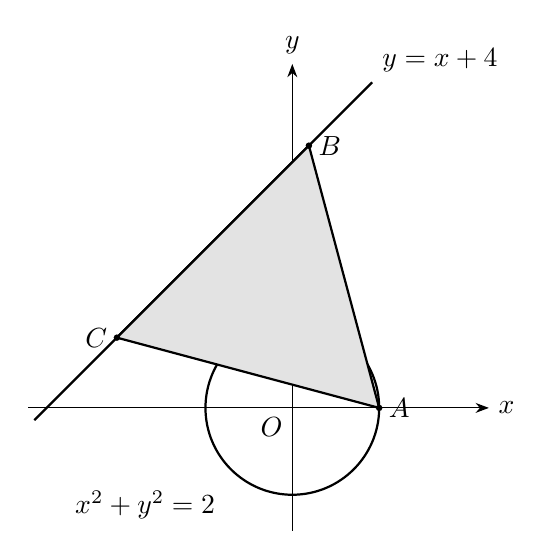
\begin{tikzpicture}[scale=0.78,>=Stealth]
  \draw[->] (-4.3,0)--(3.2,0) node[right] {$x$};
  \draw[->] (0,-2.0)--(0,5.6) node[above] {$y$};
  \draw[thick] (0,0) circle[radius=1.414];
  \draw[thick] (-4.2,-0.2)--(1.3,5.3) node[above right] {$y=x+4$};
  \coordinate (A) at (1.414,0);
  \coordinate (B) at (0.270,4.270);
  \coordinate (C) at (-2.856,1.144);
  \fill[gray!22] (A)--(B)--(C)--cycle;
  \draw[thick] (A)--(B)--(C)--cycle;
  \fill (A) circle(1.5pt) node[right] {$A$};
  \fill (B) circle(1.5pt) node[right] {$B$};
  \fill (C) circle(1.5pt) node[left] {$C$};
  \node[below left] at (0,0) {$O$};
  \node[below left] at (-1.1,-1.2) {$x^2+y^2=2$};
\end{tikzpicture}
\end{center}
\fivechoices{$4\sqrt3$}{$\dfrac{27}{4}$}{$\dfrac{20\sqrt3}{3}$}{$12$}{$12\sqrt2$}
\end{problem}

\begin{problem}{14}{5.3}
점 $A(14,2)$를 $x$축의 양의 방향으로 $a$만큼, $y$축의 양의 방향으로 $b$만큼 평행이동한 점을 $B$라 하자. 직선 $AB$가 원
\[
(x-1)^2+(y-2)^2=25
\]
과 한 점에서 만나고 $\seg{AB}=13$일 때, $ab$의 값은? (단, $a<0$, $b>0$)
\fivechoices{$-72$}{$-60$}{$-48$}{$-36$}{$-24$}
\end{problem}

\clearpage
\sectiontitle{선택형}

\begin{problem}{15}{5.5}
집합 $X=\{1,2,3,4,5,6,7,8,9,10,11,12\}$가 있다. 다음 조건을 만족시키는 집합 $X$의 두 부분집합 $A,B$에 대하여 집합 $B-A$의 모든 원소의 합은?

\begin{tcolorbox}[colback=lightblue,colframe=linegray,title={\textbf{조건}},arc=1mm]
(가) $n(A\cap B)=3$, $n(B-A)=4$\\
(나) $p\in A\cap B$이면 $\dfrac{p+2}{2}\in B-A$이다.\\
(다) $q\in B-A$이면 $q+2\in A$이다.
\end{tcolorbox}
\fivechoices{$14$}{$15$}{$16$}{$17$}{$18$}
\end{problem}

\clearpage
\sectiontitle{선택형}

\begin{problem}{16}{5.7}
그림과 같이 직선 $y=x$ 위의 점 $A$를 중심으로 하고 $x$축과 만나지 않는 원 $C$가 있다. 원점 $O$를 지나고 원 $C$에 접하는 두 직선 중 기울기가 작은 직선을 $\ell:y=mx$라 하자. 원 $C$와 직선 $y=x$의 교점 중 $x$좌표가 작은 것을 $P_1$, 큰 것을 $P_2$라 하면 $\seg{OP_1}=\sqrt2$이다. 원 $C$ 위의 점 $P_1$에서의 접선과 직선 $\ell$의 교점을 $Q_1$, 점 $P_2$에서의 접선과 직선 $\ell$의 교점을 $Q_2$라 하자. 삼각형 $AQ_2P_2$의 넓이는 삼각형 $AP_1Q_1$의 넓이의 $3$배이다. 이때 $m$의 값은? (단, 점 $A$는 제1사분면 위의 점이다.)

\begin{center}
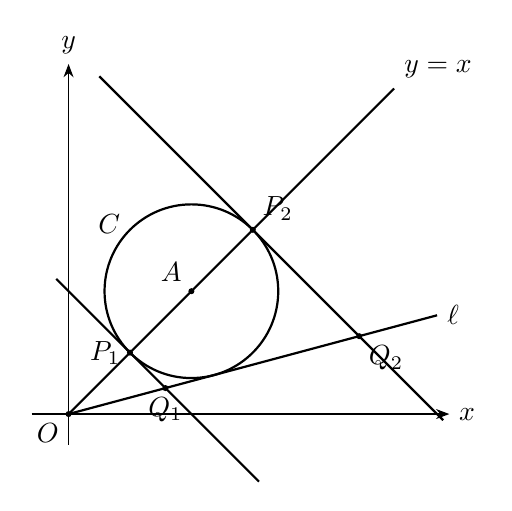
\begin{tikzpicture}[scale=0.78,>=Stealth]
  \draw[->] (-0.6,0)--(6.2,0) node[right] {$x$};
  \draw[->] (0,-0.5)--(0,5.7) node[above] {$y$};
  \draw[thick] (0,0)--(5.3,5.3) node[above right] {$y=x$};
  \draw[thick] (0,0)--(6.0,1.608) node[right] {$\ell$};
  \draw[thick] (2,2) circle[radius=1.414];
  \draw[thick] (-0.2,2.2)--(3.1,-1.1);
  \draw[thick] (0.5,5.5)--(6.1,-0.1);
  \coordinate (O) at (0,0);
  \coordinate (Pone) at (1,1);
  \coordinate (A) at (2,2);
  \coordinate (Ptwo) at (3,3);
  \coordinate (Qone) at (1.577,0.423);
  \coordinate (Qtwo) at (4.732,1.268);
  \fill (O) circle(1.4pt) node[below left] {$O$};
  \fill (Pone) circle(1.4pt) node[left] {$P_1$};
  \fill (A) circle(1.4pt) node[above left] {$A$};
  \fill (Ptwo) circle(1.4pt) node[above right] {$P_2$};
  \fill (Qone) circle(1.4pt) node[below] {$Q_1$};
  \fill (Qtwo) circle(1.4pt) node[below right] {$Q_2$};
  \node[left] at (1.0,3.1) {$C$};
\end{tikzpicture}
\end{center}
\fivechoices{$2-\sqrt3$}{$3\sqrt2-4$}{$\sqrt5-2$}{$3\sqrt3-5$}{$3-2\sqrt2$}
\end{problem}

\clearpage
\sectiontitle{선택형}

\begin{problem}{17}{5.8}
점 $A(t,1)$을 지나며 원점 $O$와의 거리가 $t$인 직선 $\ell$과 직선 $m:x=t$가 있다. 두 직선 $\ell,m$과 $x$축으로 둘러싸인 부분의 넓이를 $f(t)$라 할 때, $f(t)=\dfrac65$를 만족하는 $t$의 값은? (단, $0<t<1$)
\fivechoices{$\dfrac13$}{$\dfrac12$}{$\dfrac23$}{$\dfrac34$}{$\dfrac56$}
\end{problem}

\begin{problem}{18}{5.9}
정수 전체의 집합의 부분집합
\[
A=\left\{n-\frac{2m-1}{2},\ldots,n-\frac32,n-\frac12,
 n+\frac12,n+\frac32,\ldots,n+\frac{2m-1}{2}\right\}
\]
가 있다. 집합 $A$의 모든 원소의 합이 $k$가 되게 하는 $n(A)$의 최댓값과 최솟값의 합을 $S(k)$라 할 때,
\[
S(20)+S(40)+S(60)
\]
의 값은? (단, $m$은 자연수이다.)
\fivechoices{$260$}{$264$}{$268$}{$272$}{$276$}
\end{problem}

\clearpage
\sectiontitle{논술형}

\begin{problem}{논술형 1}{5.0}
어느 학교 학생 $50$명을 대상으로 축구와 배드민턴 활동 경험을 조사하였다. 축구 활동을 경험한 학생은 배드민턴 활동을 경험한 학생보다 $6$명 많고, 두 활동을 모두 경험한 학생은 $12$명이다. 또한 두 활동을 어느 것도 경험하지 않은 학생은 $8$명이다. 축구 활동만 경험한 학생 수와 배드민턴 활동만 경험한 학생 수를 각각 구하는 풀이 과정을 논술하시오.

\vspace{58mm}
\end{problem}

\begin{problem}{논술형 2}{7.0}
$0$이 아닌 실수 $a$에 대하여 좌표평면 위의 서로 다른 세 점 $A(4a+3,0)$, $B$, $C$가 다음 조건을 만족시킨다.
\begin{tcolorbox}[colback=lightblue,colframe=linegray,title={\textbf{조건}},arc=1mm]
\begin{itemize}[leftmargin=6mm,itemsep=1mm,topsep=0mm,bottomsep=0mm]
\item 삼각형 $ABC$의 무게중심의 좌표는 $(1,4)$이다.
\item $\seg{AB}=\seg{AC}$
\end{itemize}
\end{tcolorbox}
$\seg{BC}=2\sqrt{(2a+1)^2+4}$일 때, 점 $B$의 $x$좌표와 $y$좌표의 합을 구하는 풀이 과정을 논술하시오. (단, 점 $B$의 $x$좌표는 점 $C$의 $x$좌표보다 크다.)

\vspace{54mm}
\end{problem}

\clearpage
\sectiontitle{빠른 정답}

\renewcommand{\arraystretch}{1.55}
\begin{center}
\begin{tabular}{>{\centering\arraybackslash}m{12mm}*{6}{>{\centering\arraybackslash}m{23mm}}}
\toprule
문항 & 1 & 2 & 3 & 4 & 5 & 6\\
\midrule
정답 & ④ & ④ & ⑤ & ③ & ② & ②\\
\bottomrule
\end{tabular}

\vspace{4mm}
\begin{tabular}{>{\centering\arraybackslash}m{12mm}*{6}{>{\centering\arraybackslash}m{23mm}}}
\toprule
문항 & 7 & 8 & 9 & 10 & 11 & 12\\
\midrule
정답 & ③ & ① & ① & ③ & ① & ⑤\\
\bottomrule
\end{tabular}

\vspace{4mm}
\begin{tabular}{>{\centering\arraybackslash}m{12mm}*{6}{>{\centering\arraybackslash}m{23mm}}}
\toprule
문항 & 13 & 14 & 15 & 16 & 17 & 18\\
\midrule
정답 & ④ & ② & ⑤ & ① & ③ & ④\\
\bottomrule
\end{tabular}
\end{center}

\vspace{6mm}
\begin{tcolorbox}[colback=lightblue,colframe=navy,title={\textbf{논술형 정답}}]
\textbf{논술형 1:} 축구만 경험한 학생 $18$명, 배드민턴만 경험한 학생 $12$명\\[2mm]
\textbf{논술형 2:} $9$
\end{tcolorbox}

\clearpage
\sectiontitle{선택형 해설}

\begin{solution}{1}{④ $-1$}
$(2,1)$을 $x$축에 대하여 대칭이동하면 $(2,-1)$이다. 이를 다시 원점에 대하여 대칭이동하면 $(-2,1)$이므로
\[
a+b=-2+1=-1.
\]
\end{solution}

\begin{solution}{2}{④ $3$}
$A\subset B$가 되려면 $A$의 원소 $1,3$이 모두 $B$에 들어 있어야 한다. $1$은 이미 $B$에 있으므로 $a=3$이다.
\end{solution}

\begin{solution}{3}{⑤ $4$}
두 직선이 평행하려면 기울기가 같아야 하므로
\[
5-2k=-3.
\]
따라서 $-2k=-8$, 즉 $k=4$이다.
\end{solution}

\begin{solution}{4}{③ $16$}
$10$의 양의 약수는 $1,2,5,10$이므로
\[
A\cap B=\{1,5,10\}.
\]
모든 원소의 합은 $1+5+10=16$이다.
\end{solution}

\begin{solution}{5}{② $2$}
직선 $y=x$에 대한 대칭이동에서는 $x$와 $y$를 서로 바꾸면 된다. 따라서
\[
2x+y-4=0\quad\longrightarrow\quad x+2y-4=0.
\]
즉 $y=-\frac12x+2$이므로 $y$절편은 $2$이다.
\end{solution}

\begin{solution}{6}{② $\dfrac{\sqrt5}{3}$}
$AB$의 중점은 $\left(\frac32,\frac92\right)$이고 $AB$의 기울기는 $-1$이므로 수직이등분선은 $y=x+3$이다. $AC$의 중점은 $(0,3)$이고 $AC$의 기울기는 $2$이므로 수직이등분선은 $y=-\frac12x+3$이다. 두 직선의 교점, 즉 외심은
\[
O=(0,3)
\]
이다. 삼각형의 무게중심은
\[
G=\left(\frac{1+2-1}{3},\frac{5+4+1}{3}\right)=\left(\frac23,\frac{10}{3}\right).
\]
따라서
\[
OG=\sqrt{\left(\frac23\right)^2+\left(\frac13\right)^2}=\frac{\sqrt5}{3}.
\]
\end{solution}

\clearpage
\sectiontitle{선택형 해설}

\begin{solution}{7}{③ $10$개}
점과 직선 사이의 거리 공식으로
\[
d_1=\frac{|3m-m+3|}{\sqrt{10}}=\frac{|2m+3|}{\sqrt{10}},\qquad
d_2=\frac{|-10|}{\sqrt{10}}=\sqrt{10}.
\]
따라서
\[
|2m+3|<10\iff -10<2m+3<10\iff -\frac{13}{2}<m<\frac72.
\]
이를 만족하는 정수는 $-6,-5,\ldots,3$의 $10$개이다.
\end{solution}

\begin{solution}{8}{① $1$개}
완전제곱식으로 정리하면
\[
(x-a)^2+(y+2a)^2=2a^2-4a+3.
\]
원의 중심은 $(a,-2a)$이고 반지름은 $r=\sqrt{2a^2-4a+3}$이다. 원 전체가 제4사분면에 있으려면 특히 왼쪽 끝점이 $y$축의 오른쪽에 있어야 하므로 $a-r>0$이어야 한다. 이 조건이면 $a>0$이고 $r<a<2a$이므로 원의 위쪽 끝점도 $x$축 아래에 있다. 따라서
\[
r<a\iff 2a^2-4a+3<a^2
\iff (a-1)(a-3)<0.
\]
즉 $1<a<3$이고 정수 $a$는 $2$ 하나뿐이다.
\end{solution}

\begin{solution}{9}{① $-50$}
원 $x^2+y^2=25$ 위의 점 $(3,4)$에서의 접선은
\[
3x+4y=25
\]
이다. 두 번째 원은
\[
(x-1)^2+(y+7)^2=50-k
\]
이므로 중심은 $(1,-7)$이다. 중심에서 접선까지의 거리는
\[
\frac{|3-28-25|}{5}=10.
\]
접하려면 반지름이 $10$이어야 하므로
\[
50-k=100,\qquad k=-50.
\]
\end{solution}

\begin{solution}{10}{③ $16$}
$B\cup X=B$이므로 $X\subset B$이다. 또한 $A\cap X=\varnothing$이므로
\[
X\subset B-A.
\]
여기서
\[
A=\{1,2,3,6\},\qquad B=\{3,6,9,12,15,18\}
\]
이므로 $B-A=\{9,12,15,18\}$이다. 따라서 가능한 $X$는 네 원소로 이루어진 집합의 모든 부분집합이므로
\[
2^4=16
\]
개이다.
\end{solution}

\clearpage
\sectiontitle{선택형 해설}

\begin{solution}{11}{① $-\dfrac43$}
두 직선의 교점의 $x$좌표를 구하면
\[
-\frac13x+5=kx-3k+2
\]
에서
\[
(3k+1)x=9(k+1),\qquad x=\frac{9(k+1)}{3k+1}.
\]
교점이 제2사분면에 있으면 $x<0$이어야 한다. 이때 첫 번째 직선에서 $y=-\frac13x+5>0$이 자동으로 성립하므로
\[
\frac{k+1}{3k+1}<0.
\]
따라서
\[
-1<k<-\frac13.
\]
즉 $a=-1$, $b=-\frac13$이므로 $a+b=-\frac43$이다.
\end{solution}

\begin{solution}{12}{⑤ $5\sqrt2$}
$Q=(q,0)$라 하면 $P=(q-1,0)$이다. $A'=(-1,4)$라 놓으면 평행이동에 의해
\[
AP=A'Q.
\]
또 $A'$를 $x$축에 대하여 대칭이동한 점을 $A''=(-1,-4)$라 하면 $A'Q=A''Q$이다. 따라서 고정된 $B$에 대하여
\[
AP+QB=A''Q+QB
\]
의 최솟값은 선분 $A''B$가 $x$축과 만날 때의 $A''B$이다. 원 $C$의 중심을 $O_C=(5,2)$라 하면
\[
A''O_C=\sqrt{6^2+6^2}=6\sqrt2,\qquad r=\sqrt2.
\]
그러므로 $B$까지의 최단거리는
\[
6\sqrt2-\sqrt2=5\sqrt2.
\]
\end{solution}

\begin{solution}{13}{④ $12$}
점 $A$에서 직선 $y=x+4$, 즉 $x-y+4=0$까지의 거리를 $d$라 하자. 정삼각형의 높이가 $d$이므로 한 변의 길이는 $\frac{2d}{\sqrt3}$이고 넓이는
\[
\frac{\sqrt3}{4}\left(\frac{2d}{\sqrt3}\right)^2=\frac{d^2}{\sqrt3}
\]
이다. 원 $x^2+y^2=2$ 위에서는 $x-y$의 최댓값과 최솟값이 각각 $2,-2$이므로
\[
\sqrt2\le d=\frac{x-y+4}{\sqrt2}\le 3\sqrt2.
\]
따라서
\[
m=\frac{(\sqrt2)^2}{\sqrt3}=\frac2{\sqrt3},\qquad
M=\frac{(3\sqrt2)^2}{\sqrt3}=6\sqrt3.
\]
그러므로 $M m=12$이다.
\end{solution}

\begin{solution}{14}{② $-60$}
원의 중심을 $O=(1,2)$라 하면 $AO=13$이고 반지름은 $5$이다. 직선 $AB$는 원의 접선이므로 $A$에서 접점까지의 거리는
\[
\sqrt{13^2-5^2}=12.
\]
또 $\vect{AB}=(a,b)$이고 $AB=13$이다. 중심 $O$에서 직선 $AB$까지의 거리가 반지름 $5$이므로, $AO$가 수평인 점을 이용하면 이 거리는 $|b|$이다. $b>0$이므로 $b=5$이다. 따라서
\[
a^2+b^2=13^2\implies a^2=144.
\]
$a<0$이므로 $a=-12$이고 $ab=-60$이다.
\end{solution}

\clearpage
\sectiontitle{선택형 해설}

\begin{solution}{15}{⑤ $18$}
$C=A\cap B$, $D=B-A$라 놓자. 조건 (나)에 의해 $p\in C$이면 $\frac{p+2}{2}\in D$이므로 $p$는 짝수이다. $p=2$이면 그 상이 다시 $2$가 되어 $C\cap D=\varnothing$에 모순이므로
\[
C\subset\{4,6,8,10,12\}.
\]
또 $p$와 $p+4$가 함께 $C$에 있으면 그 상은 서로 $2$만큼 차이나는 두 원소로서 $D$에 들어간다. 그런데 조건 (다)에 의해 $q\in D$이면 $q+2\in A$이므로 $q+2$가 다시 $D$에 있을 수 없다. 또한 $4,6$이 함께 $C$에 있으면 $6$의 상인 $4$가 $D$에도 들어가고, $6,10$이 함께 $C$에 있어도 같은 모순이 생긴다. 세 원소를 고를 수 있는 경우를 점검하면
\[
C=\{4,10,12\}
\]
만 가능하다. 조건 (나)로부터
\[
\{3,6,7\}\subset D.
\]
$D$의 네 번째 원소를 $q$라 하자. 조건 (다)와 $C\cap D=\varnothing$을 함께 적용하면 $q=2$만 가능하다. 실제로
\[
D=\{2,3,6,7\}
\]
이고 모든 조건을 만족한다. 따라서 원소의 합은 $2+3+6+7=18$이다.
\end{solution}

\begin{solution}{16}{① $2-\sqrt3$}
$P_1$은 직선 $y=x$ 위에 있고 $OP_1=\sqrt2$이므로 $P_1=(1,1)$이다. $P_2=(p,p)$라 놓으면 중심 $A$는 지름 $P_1P_2$의 중점이다. $P_i=(u,u)$에서 원의 접선은 기울기가 $-1$이므로
\[
P_1\text{에서의 접선}:y=-x+2,\qquad
P_2\text{에서의 접선}:y=-x+2p.
\]
이들을 $\ell:y=mx$와 만나게 하면 $Q_2$의 좌표는 $Q_1$의 좌표의 $p$배이다. 두 삼각형 $AP_1Q_1$, $AQ_2P_2$는 밑변 $AP_1$, $AP_2$의 길이가 같고, $Q_2$에서 직선 $y=x$까지의 거리가 $Q_1$의 거리의 $p$배이므로 넓이의 비도 $p:1$이다. 주어진 조건에 따라 $p=3$이다.

따라서 $P_2=(3,3)$, $A=(2,2)$이고 원의 반지름은 $AP_1=\sqrt2$이다. 직선 $mx-y=0$이 원에 접하므로
\[
\frac{|2m-2|}{\sqrt{m^2+1}}=\sqrt2.
\]
이를 제곱하여 정리하면
\[
m^2-4m+1=0,\qquad m=2\pm\sqrt3.
\]
두 접선 중 기울기가 작은 것을 택하므로 $m=2-\sqrt3$이다.
\end{solution}

\begin{solution}{17}{③ $\dfrac23$}
직선 $\ell$의 기울기를 $s$라 하면, 점 $A(t,1)$을 지나므로
\[
\ell:y-1=s(x-t),\qquad sx-y+1-st=0.
\]
원점에서 이 직선까지의 거리가 $t$이므로
\[
\frac{|1-st|}{\sqrt{s^2+1}}=t.
\]
$0<t<1$인 상황에서 제곱하여 정리하면
\[
1-2st=t^2,\qquad s=\frac{1-t^2}{2t}.
\]
직선 $m:x=t$와 $x$축, $\ell$이 만드는 삼각형의 높이는 $1$이고 밑변은 $1/s$이므로
\[
f(t)=\frac12\cdot\frac1s\cdot1=\frac{t}{1-t^2}.
\]
따라서
\[
\frac{t}{1-t^2}=\frac65
\iff 6t^2+5t-6=0
\iff (3t-2)(2t+3)=0.
\]
$0<t<1$이므로 $t=\frac23$이다.
\end{solution}

\begin{solution}{18}{④ $272$}
집합 $A$에는 $2m$개의 원소가 있고, 원소들은 $n$을 중심으로 대칭이므로 원소의 합은
\[
2mn=k.
\]
또 모든 원소가 정수이고 각 원소가 $n$에서 반정수만큼 떨어져 있으므로 $2n$은 홀수이다. 따라서
\[
\frac{k}{m}=2n
\]
은 홀수여야 한다. 즉 $m$은 $k$의 약수 중 $k/m$이 홀수인 값이다.

\begin{itemize}[leftmargin=7mm,itemsep=1mm]
\item $k=20$: $m=4,20$, 따라서 $n(A)=8,40$이고 $S(20)=48$.
\item $k=40$: $m=8,40$, 따라서 $n(A)=16,80$이고 $S(40)=96$.
\item $k=60$: $m=4,12,20,60$, 따라서 $n(A)=8,24,40,120$이고 $S(60)=128$.
\end{itemize}
그러므로
\[
S(20)+S(40)+S(60)=48+96+128=272.
\]
\end{solution}

\clearpage
\sectiontitle{논술형 해설}

\begin{solution}{논술형 1}{축구만 $18$명, 배드민턴만 $12$명}
축구 활동만 경험한 학생 수를 $x$, 배드민턴 활동만 경험한 학생 수를 $y$라 하자. 두 활동을 모두 경험한 학생은 $12$명, 어느 것도 경험하지 않은 학생은 $8$명이므로
\[
x+y+12+8=50,
\]
즉 $x+y=30$이다. 축구 활동 경험자는 $x+12$명, 배드민턴 활동 경험자는 $y+12$명이고 전자가 후자보다 $6$명 많으므로
\[
(x+12)-(y+12)=6,
\]
즉 $x-y=6$이다. 두 식을 연립하면
\[
x=18,\qquad y=12.
\]
따라서 축구 활동만 경험한 학생은 $18$명, 배드민턴 활동만 경험한 학생은 $12$명이다.
\end{solution}

\begin{solution}{논술형 2}{$9$}
$B=(x_1,y_1)$, $C=(x_2,y_2)$라 하고 $BC$의 중점을 $M$이라 하자. 삼각형의 무게중심이 $(1,4)$이므로
\[
\frac{(4a+3)+x_1+x_2}{3}=1,\qquad
\frac{y_1+y_2}{3}=4.
\]
따라서
\[
x_1+x_2=-4a,\qquad y_1+y_2=12,\qquad M=(-2a,6).
\]
$AB=AC$이므로 $AM$은 $BC$의 수직이등분선이다. 벡터
\[
\vect{AM}=(-2a-(4a+3),6)=(-6a-3,6)=3\bigl(-(2a+1),2\bigr)
\]
에 수직인 방향벡터로 $(2,2a+1)$을 잡을 수 있다. 주어진 $BC$의 길이는
\[
2\sqrt{(2a+1)^2+4}=2\left\|(2,2a+1)\right\|
\]
이므로 중점 $M$에서 두 끝점까지의 벡터는 서로 반대인 $\pm(2,2a+1)$이다. 점 $B$의 $x$좌표가 더 크므로
\[
B=M+(2,2a+1)=(2-2a,\,2a+7).
\]
따라서 점 $B$의 두 좌표의 합은
\[
(2-2a)+(2a+7)=9.
\]
\end{solution}

\vfill
\begin{center}
{\small 원본의 파란색 정답 표시를 참고하되, 모든 답은 별도로 계산하여 검증하였습니다.}
\end{center}

\end{document}
